\documentclass[conference]{IEEEtran}
\usepackage{amsmath,amssymb,booktabs,graphicx,balance}
\usepackage[hidelinks]{hyperref}
\hypersetup{pdftitle={Sharing Retained Git Events in a Graph Memory for Coding Agents},pdfauthor={Anonymous working draft}}
\usepackage{iftex}
\ifXeTeX
\usepackage{fontspec}
\setmainfont{texgyretermes-regular.otf}[BoldFont=texgyretermes-bold.otf,ItalicFont=texgyretermes-italic.otf,BoldItalicFont=texgyretermes-bolditalic.otf]
\setsansfont{texgyreheros-regular.otf}[BoldFont=texgyreheros-bold.otf,ItalicFont=texgyreheros-italic.otf]
\setmonofont{texgyrecursor-regular.otf}[BoldFont=texgyrecursor-bold.otf]
\fi
\title{Sharing Retained Git Events in a Graph Memory for Coding Agents}
\author{\IEEEauthorblockN{Anonymous working draft}}
\begin{document}
\maketitle
\begin{abstract}
A coding agent can use past changes to choose another file to inspect. An event store preserves which files changed together, which file kept the event, and which inputs justified a recommendation. Our demonstration lets visitors expand the source events, compare two storage plans that recover the same answer, and switch between histories with identical pair counts but different answers to a two-file query. In an independent replay of 932 one-file queries, favoring small events reduced decoded member bytes by 33.1\% at the same number of decoded events. The mean project-level change in Recall@8 was $+0.33$ percentage points (95\% interval $[-0.57,+1.43]$). On 621 two-file queries, adding evidence that all three files co-occurred reached 37.19\% recall, versus 36.89\% for summed pair weights and 37.82\% for a control that redistributed the same evidence mass. Across 196 exact reads on the same compact complete index, sharing cached events transferred 21,142 bytes versus 123,058 with owner-only reads. Discarding volatile memory midstream raised this to 106,781 bytes. The demonstration makes these tradeoffs inspectable on individual decisions.
\end{abstract}

\section{Who still holds the evidence?}
A coding agent opens a graph generator and needs to decide which test to read. The generator's latest changes concern utilities used throughout the project. Its test changed with the generator in earlier commits. The generator may have exhausted its retention budget while the less frequently modified test still holds those earlier events. A second question arises when the agent already knows two implementation files. Did a candidate test change with each file on separate occasions, or did all three appear in the same change? A table of pair weights can give the same answer in both situations.

ROSE~\cite{zimmermann} established version histories as a source of file recommendations. Moonen et al.~\cite{moonen} showed empirically that a cutoff on transaction size can improve association-rule recommendations. Higher-order link prediction also distinguishes co-membership in one interaction from the corresponding pair projection~\cite{benson}. Temporal graph systems for agents such as TAPE~\cite{tape} make dated relationships queryable. Our system lets a visitor change the read policy over a fixed event store, inspect the commits added to an answer, and see when the answer can be reconstructed by a smaller representation. In particular, we investigate the joint effects of retaining an event on behalf of several files, reading it through an anchor that has evicted it, and evaluating whether this changes which file the agent should inspect.

\begin{figure}[t]
\centering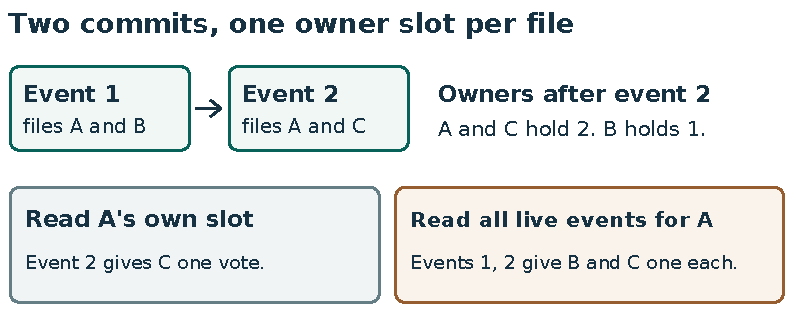
\includegraphics[width=\columnwidth]{retention.pdf}
\caption{After file A evicts its reference to event 1, file B still holds it. The live incidence index points from A to both events.}
\label{fig:retention}
\end{figure}

An immutable event supplies concrete provenance for every added vote. The Git reader uses revision identifiers and paths observed to change on successive first-parent transitions. This permits operation without a whole-repository embedding pass or access to source contents. It also limits what the ranking can infer about semantically related files with no common history. The prototype provides an offline replay and a SQLite console. Visitors can restore a particular prefix, compare retrieval budgets, or expose the information lost in a projection. The interface distinguishes source availability, sufficient information for exact ranking, and agreement with the next observed change.

\section{Retention, projection and recovery}
\subsection{Write an event once}
For an accepted Git event $e$, $M_e$ is its set of Python paths and the commit SHA identifies its source. Paths receive integer IDs at their first appearance. Events with 2--64 paths form the co-edit history. Single-file commits can still contribute to recent frequency. Let $O_t(f)$ contain the last $b$ accepted events involving file $f$, with $b=8$. The hot set and the events readable through anchor $a$ are
\[
 H_t=\bigcup_f O_t(f),\qquad I_t(a)=\{e\in H_t:a\in M_e\}.
\]
When a path advances its queue, a released event remains hot as long as another member still owns it. An incidence index identifies all members of a surviving event. One new event with $m$ paths introduces $m$ incidences. Expanding it into directed pair counts would generate $m(m-1)$ updates. The queues, live incidence index and historical archive have separate storage costs.

For a one-file query, each decoded event that contains $a,x$ gives $x$ a vote. The reader may count events, or give each pair weight $1/(|M_e|-1)$ so that one known participant distributes one unit over its partners~\cite{newman}. The ties use file frequency in the preceding 32 commits and then the first-seen ID. An owner-only reader uses $O_t(a)$. A shared reader can use all of $I_t(a)$, or inspect event sizes before choosing which eight bodies to read. Size selection requires access to member-count metadata even when it avoids decoding the bodies themselves.

\subsection{Which exact query can an index answer?}
The exact one-file reader must return the same ordered eight IDs \emph{and their scores} as the complete relevant history of raw co-edit counts. A partition of historical events into hot and evicted sets lets a query sum the two contributions. For $D$ fully evicted events, let $d_f$ be the number that contained $f$ and $v$ the visible count for pair $a,x$. Inclusion--exclusion in this common universe bounds the full count:
\[
v+\max(0,d_a+d_x-D)\ \le s(a,x)\le\
v+\min(d_a,d_x).
\]
When a candidate's score is fixed and no competitor's upper key can displace it under the tie rules, it may be certified without checking the archive. An offline evaluator uses these bounds. The timed shared SQLite reader applies the simpler sufficient condition $d_a=0$ and otherwise reads the required archived events. Key equality after recovery and exactness known before recovery are separately measurable.

For each of two observed files $a,b$, the reader prefers recent surviving events of size at most six and fills up to eight by recency. It takes the union and decodes each event once. For another file $x$, the normalized sum of the pair weights is $p(x)$. A joint event with $a,b,x$ contributes $1/(|M_e|-2)$ to $q(x)$. We compare the rank of $p(x)+q(x)$ with the pair sum alone. A control redistributes the same joint-event mass by the harmonic mean of the two pair weights. It keeps the total joint-event count and discards its candidate-specific assignment. All three rankings share events, candidates and tie rules.

One can also ask whether the two-anchor answer is already determined by aggregated counts. Divide selected events into strata by size $m$. Let $J_m$ count events containing both anchors, and $t_x$ count such events also containing candidate $x$. Each joint event has exactly $m-2$ other members. Consequently $\sum_x t_x=J_m(m-2)$ within a stratum. The solver bounds each $t_x$ by the observed separate counts for $(a,x)$ and $(b,x)$ and tightens the bounds using this sum. It refines unresolved scores by reading joint events in selected strata. This certificate assumes the query-specific counts and event addresses are available.

\begin{figure*}[t]
\centering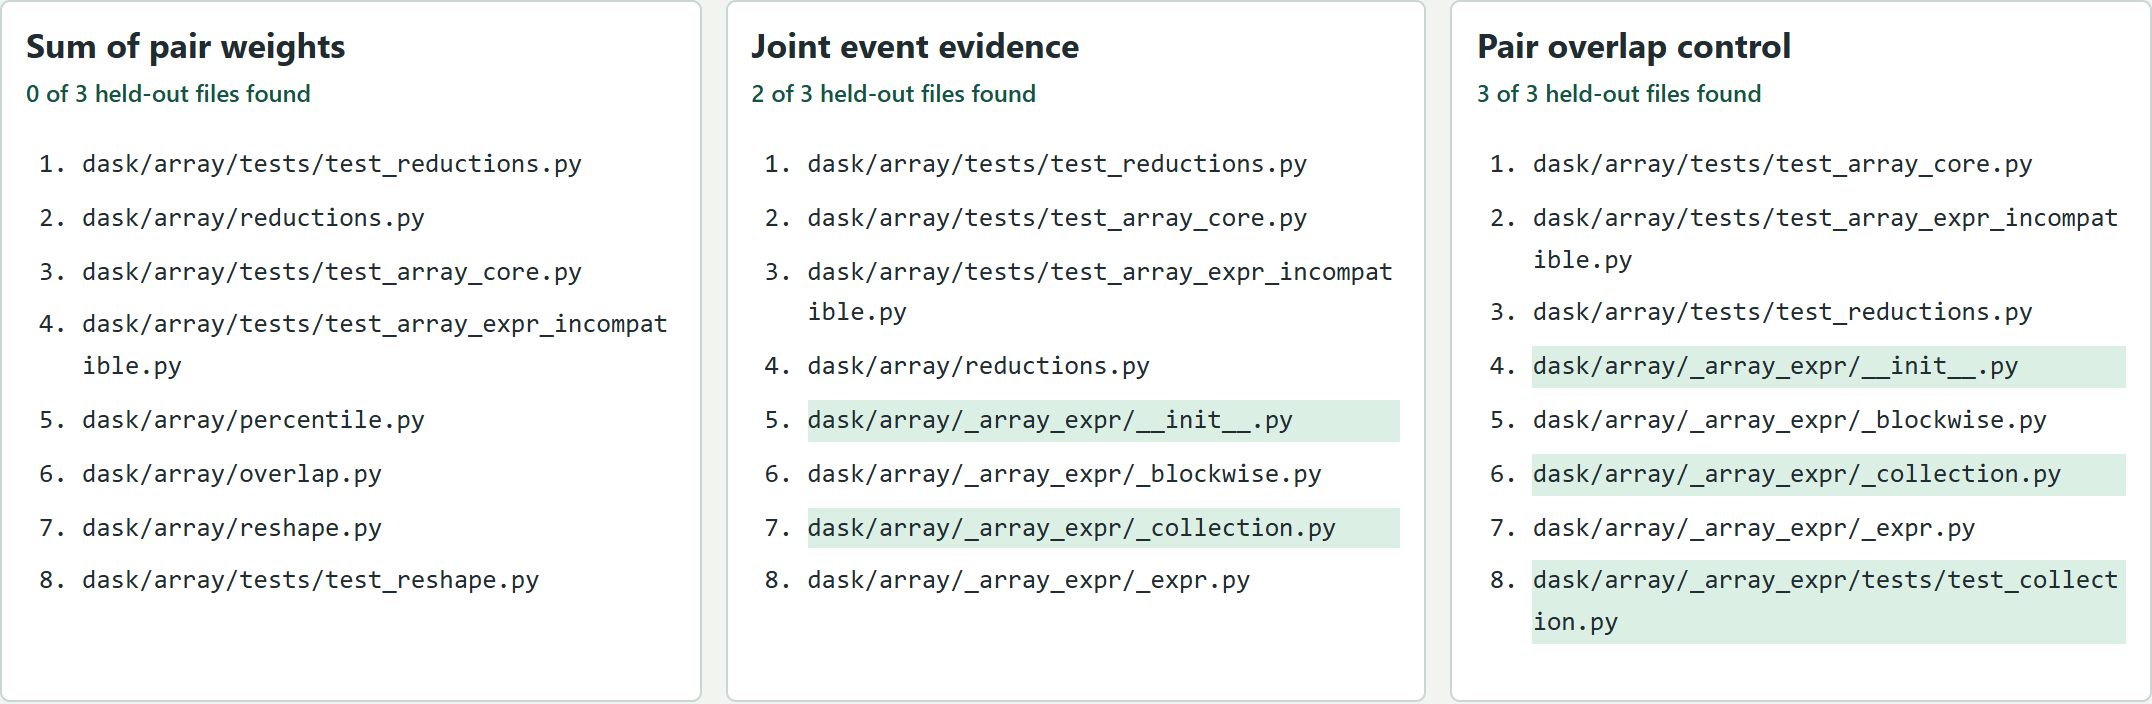
\includegraphics[width=.99\textwidth]{dask-replay.png}
\caption{Results displayed by the SQLite replay before Dask commit \texttt{06c1bb72}. The three cards use identical historical events. The pair sum covers zero of three held-out files, preserving their candidate-specific joint occurrences covers two, and using pair overlap and the joint-event count covers all three. The visitor can hide the annotations or expand the contributing commits beneath the table.}
\label{fig:dask}
\end{figure*}

\section{Visitor scenarios}
\subsection{Track the lifetime of a test's evidence}
Open the directed-generator case in the English replay. In the owner-only view, the eight events contain 252 file memberships. In the shared view, 15 events contain 421 memberships. Four additional commits mention the actual test, moving \texttt{test\_directed.py} to rank five with six votes. Expanding \texttt{539ad536} shows that the test itself retained a source that the generator had evicted. Each commit is linked back to Git; the snapshot and rankings are available offline.

Switch to the HITS implementation before NetworkX commit \texttt{1e5933df}. With eight owner events the actual test ranks fourth with four votes. Reading 23 shared events adds two votes to the same test. Competing files gain even more and it drops outside the eight suggestions. Visitors can inspect the identities of all 15 additional events, including those that failed to support the test. The examples deliberately exhibit opposite outcomes.

\subsection{Give the agent two known files}
Open \texttt{seed\_pair/demo.html} offline, or run \texttt{demo.py serve} in its directory and choose the live SQLite source. The console lets a visitor choose a real commit, inspect the two revealed paths and compare distinct uses of the same source records. Before Dask commit \texttt{06c1bb72} (Fig.~\ref{fig:dask}), the known paths are the array package initializer and its expression module \texttt{\_io.py}. Of the three held-out paths, the pair sum finds zero, candidate-specific joint evidence finds two, and redistributing the same joint mass by harmonic pair support finds all three. For xarray commit \texttt{503b262d}, the pair sum recovers one of two targets while the joint score recovers neither. Visitors can inspect the history rows that support each candidate, then reveal the reference targets to annotate the predicted order.

Switch from a real commit to two constructed histories (Fig.~\ref{fig:pair}). For three groups $A,B,C$ each of size $n$, history $s$ consists of events $(A_i,B_j,C_{(i+j+s)\bmod n})$. Every cross-group pair appears once for every $s$. The visitor may compare pair counts across histories before opening the event for $(A_i,B_j)$. A change of $s$ changes its third file while every pair count is preserved. Across uniformly weighted histories any method with only these pair counts has expected Hit@$k\le k/n$ for $k\le n$. The $n=16$ replay has 768 equal pair counts across worlds, 256 queries per world and 4,096 in total. At $k=8$ the pair-only ceiling is 2,048 hits; preserved events identify all 4,096 third members. File-pair timestamps or event identifiers may retain the missing information and fall outside that bound.

\begin{figure}[t]
\centering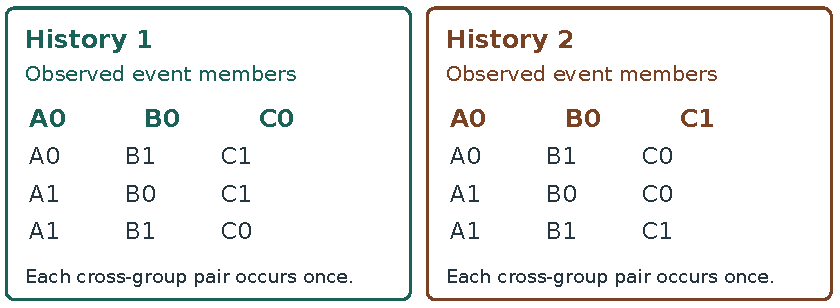
\includegraphics[width=\columnwidth]{pair-worlds.pdf}
\caption{Two possible histories, shown at $n=2$. The bold rows give different third members for the same known files. Every individual pair of files across the three groups has the same count in the two histories.}
\label{fig:pair}
\end{figure}

\subsection{Check an alternative physical plan}
The durable reader appends ordered members and the revision identity in a SQLite transaction. One representation maintains hot ownership and records a file's postings in the cold index when an event loses its last owner. On reopening, replaying the live events in chronological order reconstructs the file queues, because every path's most recent $b$ events belong to their union. A second representation keeps \emph{all} event IDs per file as a compact posting list. An archive query through either can reconstruct the complete one-anchor result. The physical comparison includes a restart check and identical retries. All experiments use a single writer. An event is immutable after it has been acknowledged.

\section{Measured costs and predictive utility}
\subsection{Replicating one-file selection}
We predict companion paths from the Git prefix before a held-out multi-file commit is inserted. Recall@8 is the fraction of other paths in the commit among the eight returned; previously unseen targets remain in the denominator. On a discovery panel of 196 queries over three 4,096-commit histories, reading every shared event raised recall from 41.97\% to 43.53\% while increasing the number of events decoded from 1,258 to 4,988. The gain varied by project from $-0.17$ to $+4.63$ points. The eight smallest available events gave 45.88\%. A subsequent size-based control motivated a separate replication.

\begin{table}[t]
\caption{Independent one-anchor panel. Both ranking weights and size thresholds were held fixed before evaluating 932 queries. Macro recall gives each project equal weight. The byte count measures decoded member IDs.}
\label{tab:replication}\centering\small
\setlength{\tabcolsep}{3.5pt}
\begin{tabular}{@{}lrrrr@{}}\toprule
Weighted read & Macro R@8 & Pooled R@8 & Events & Bytes \\\midrule
Last eight & 58.39\% & 61.76\% & 5,953 & 280,888\\
Size $\le6$, then fill & 58.72\% & 62.58\% & 5,953 & 187,864\\
Strict size $\le6$ & 59.45\% & 62.56\% & 4,737 & 60,196\\
Strict size $\le8$ & 59.29\% & 63.24\% & 5,060 & 73,524\\\bottomrule
\end{tabular}
\end{table}

On six new repositories, 932 one-anchor queries tested the frozen size rule (Table~\ref{tab:replication}). Both main arms give each pair the same inverse-size weight. The challenge arm prioritizes the newest available events containing at most six paths, filling any remaining slots by recency. The control reads the anchor's last eight. Across identical numbers of decoded events the new rule reduced decoded member bytes by 33.1\%. The mean project-level recall difference was $+0.33$ points, paired 95\% bootstrap interval $[-0.57,+1.43]$ across six projects. Per query there were 44 wins, 54 losses and 834 ties. The literal size cutoffs adapted from Moonen et al. were competitive and read substantially fewer bodies. The modeled bytes exclude metadata discovery, queue maintenance and the cost of applying the policy.

\subsection{Comparing complete durable representations}
A byte-efficient complete index is a strong baseline (Table~\ref{tab:storage}). Every representation preserves the full SHA and original ordered file IDs. The split layout stores textual SHA and fixed-width members. The packed posting implementation stores binary SHA, unsigned variable-length members and a chronological variable-length posting list per file. Both expose the same exact one-file answer and reversible event receipt. Filesystem sizes are summed after a WAL checkpoint and truncation across the three long-panel projects. Common path dictionaries and tie metadata are external to these measurements. Each write is one SQLite transaction with FULL synchronous mode. Comparing the split and packed layouts varies both index and codec. The four complete file-list variants use identical persistent bytes.

\begin{table}[t]
\caption{Exact one-anchor reads on 196 long-panel queries. Disk is checkpointed database size. The last two columns are total posting and event bytes delivered at query time, with continuous operation or a midstream restart. Restart reconstruction is charged separately.}
\label{tab:storage}\centering\small
\setlength{\tabcolsep}{4pt}
\begin{tabular}{@{}lrrr@{}}\toprule
Plan & Disk bytes & Continuous & Restart \\\midrule
Complete file lists & 323,584 & 149,294 & 149,294\\
Lists + read-through LRU & 323,584 & 91,732 & 102,444\\
Lists + own events & 323,584 & 123,058 & 128,801\\
Lists + shared events & 323,584 & 21,142 & 106,781\\
Durable hot/cold split & 512,000 & 27,716 & 27,716\\\bottomrule
\end{tabular}
\end{table}

On the identical 323,584-byte file lists, serving an anchor from every event still retained by any owner transferred 12,692 posting bytes and 8,450 event-body bytes under uninterrupted operation. Serving only the anchor's own events transferred 123,058 bytes in total. Over five paired blocks the median query time fell from 38.36 to 28.50 ms, at identical sampled cache footprints. Write-plus-cache-plus-read time changed from 2.412 to 2.400 s. A read-through LRU maintaining exact counts for cached anchors transferred 91,732 bytes and took 31.61 ms; across the three projects its sampled peak Python footprint totaled 1.32 MB, versus 5.29 MB for the owning caches. After a midstream reset the shared-content plan needed 106,781 query bytes, while the durable split restored 51,120 bytes outside its query path and then served 27,716. All plans returned identical IDs and scores. In a separate unbounded anchor-cache control, read-through LRU still transferred 91,732 bytes after restart, below the cold shared cache.

The durable split was faster (19.62 ms warm, 20.36 ms after reopening, 2.347 s mixed). A cold volatile shared cache took 37.29 ms. On 880 warm queries in six other projects, compact owner-only/shared reads transferred 25,727/6,349 bytes. Eight-event source frames reduced long-panel disk size to 303,104 bytes (299,008 versus 319,488 after vacuuming) while increasing event bytes read from 135,845 to 463,669. On the other panel frames occupied more space.

The two-anchor certificate determined 1,120 of 1,153 exact ranked outputs without archive access. Resolving the other 33 took 43 of 1,676 eligible joint events. Every final answer matched full reconstruction. Transmitting fixed-width counters and refinements cost 535,143 bytes versus 392,416 for all selected events; comparable variable-length codecs retained this ordering. Savings in archive access presuppose available query-specific counters.

\balance
\subsection{Which improvements reach a coding agent?}
On an independent two-anchor panel, 621 queries from six additional repositories yielded pooled Recall@8 of 36.89\% for the pair sum, 37.19\% for candidate-specific joint votes and 37.82\% for the mass-matched harmonic control. A joint event was available in 314 queries. The joint-versus-sum change averaged $+0.17$ points by repository with interval $[-1.17,+1.42]$. The mathematical construction establishes what pair counts can lose. The controlled real data leave the quality benefit of storing candidate-specific three-way evidence unresolved.

On Agent Retrieval Bench~\cite{arb}, we reproduced official Recall@5 for seven published rankings on all 106 canonical code-to-test tasks. On the inherited experimental panel of 105 tasks, adding a history-based fifth suggestion to role-filtered Qwen3-Embedding-4B changed recall from 68.98\% to 69.62\%, interval for the difference $[-2.58,+3.30]$ points. Only seven of 33 multi-path tasks contained a usable past event connecting multiple known paths to a test. On the same strong ensemble, prioritizing explicit joint support reduced recall from 78.03\% to 77.56\%. Enforcing exactly five new addresses in both arms left the aggregate scores unchanged. In a separate pilot covering 36 masked functions, Qwen3-4B-Instruct-2507 passed all example tests on 15 functions with recently co-edited tests and on 15 with full-history BM25 selection. These evaluations address file discovery and short executable examples.

We also replayed 108 released SWE-agent~\cite{sweagent} trajectories from GPT-4 and Claude 3.5 Sonnet on the same 54 SWE-bench Verified issues. Among 134 observed returns to a previously visited file after viewing a different one, shared event memory, own-only memory and choosing the most recent alternative file all achieved 109 top-one hits. Extra links increased historical events inspected from 219 to 271. Under a 16\,KiB content budget on 822 real editor views, a graph-aware cache served 327,334 previously observed bytes. A two-level file/line LRU reproduced the same service at every view. These measurements preserve the recorded trajectory. Effects on the behavior and success of an agent operating with a different memory remain open.

\section*{Acknowledgments}
OpenAI Codex drafted and revised the paper, implemented and exercised the prototypes, and analyzed the archived outputs. The replication materials include the frozen policies, per-query decisions and checks against independently reconstructed histories.

\bibliographystyle{IEEEtran}
\bibliography{sources}
\end{document}
